\markboth{Discharge curves}{Discharge curves}
\section{Discharge curves} \label{sec:dischargeCurves}
Many battery data sheets provide measured discharge curves, on which the charging and discharging behaviour of this model is based. Rather than determining the curves according to the internal impedance, a common approach \cite{lijun_gao_dynamic_2002}, this model determins the curves directly by means of digitizing the images and creating a curve fit. The classes used for fitting and modelling the discharge curves are described in the following subsections.

\subsection{Single discharge curve}
For modelling a single discharge curve, the class \mcode{dischargeFit} is used, which implements the interface \mcode{curveFitInterface}\todo{Section describing interface, etc.}. The curve is fitted according to \cite{werder_entwicklung_2014}, using a function that is loosely based on the Nernst equation with two exonential functions superimposed as a correction for the voltage drops at the beginning and end of the curve.
\begin{equation}
\begin{aligned}
V(SoC) = x_1 - \frac{R\cdot T}{z\subi{Li}\cdot F}\cdot ln\Big(\frac{SoC}{1-SoC}\Big)
+ x_2\cdot SoC + x_3 \\
+ (x_4 + (x_5 + x_4\cdot x_6)\cdot SoC)\cdot exp(-x_6\cdot SoC) \\
+ x_7\cdot exp(-x_8\cdot SoC)
\end{aligned}
\end{equation}

where $x_1,\ ..,\ x_8$ are the fit parameters, $R = 8.3144598$ J/(mol $\cdot$ K) is the universal gas constant, $z\subi{Li} = 1$ is the ionic charge number of lithium, $F = 96485.3328959$ As/mol is the Faraday constant, $SoC$ is the state of charge, $V$ is the voltage in V and $T$ is the temperature in K at which the curve was recorded. The curves are fitted using the levenberg-marquardt algorithm and either the \mcode{lsqcurvefit} method, the \mcode{fminsearch} method or a combination of both, depending on the user's preference. 

\subsubsection{Object creation}
A \mcode{dischargeFit} object is created with the digitized raw data - the voltage $V$ in V, the discharge capacity $C\subi{dis}$ in Ah, the current $I$ in A at which the curve was recorded and the temperature $T$ in K at which the curve was recorded.
\begin{lstlisting}
d = dischargeFit(V, C_dis, I, T);
\end{lstlisting}
\mcode{V} and \mcode{C_dis} are vectors containing the digitized raw data from the data sheet. Further options, such as initial values for the fit parameters $x_1,\ ..,\ x_8$ and the fit method can be passed to the constructor using Matlab's name-value pair syntax:
\begin{lstlisting}
d = dischargeFit(V, C_dis, I, T, 'OptionName', OptionValue);
\end{lstlisting}
By default, the initial fit parameters are set to zero and the curve is fit by first using \mcode{lsqcurvefit}, followed by \mcode{fminsearch}. The initial fit parameters are stored in a vector \mcode{x0} of \mcode{length} 8, which can be passed via the option name \mcode{'x0'}, for example using the following syntax:
\begin{lstlisting}
x0 = ones(8, 1);
d = dischargeFit(V, C_dis, I, T, 'x0', x0);
\end{lstlisting}
The method used for the curve fitting can be passed to the constructor using the option name \mcode{'mode'}. The corresponding value must be one of the following three strings:
\begin{itemize}
	\item \mcode{'lsq'} for \mcode{lsqcurvefit}
	\item \mcode{'fmin'} for \mcode{fminsearch}
	\item \mcode{'both'} for \mcode{lsqcurvefit} followed by another fit using \mcode{fminsearch}
\end{itemize}
e.g.
\begin{lstlisting}
d = dischargeFit(V, C_dis, I, T, 'mode', 'fmin');
d.plotResults
\end{lstlisting}
Depending on the curve and on the technology, one of the methods may return a better result.

\subsubsection{Visual validation}
A visual validation can be performed by calling the class's \mcode{plotResults} method (see above). In Figure~\ref{fig:dischargeFit01}, the results of two \mcode{dischargeFit} objects using the same raw data are compared.
\begin{figure}[b!]
	\captionsetup{type=figure}
	\centering
	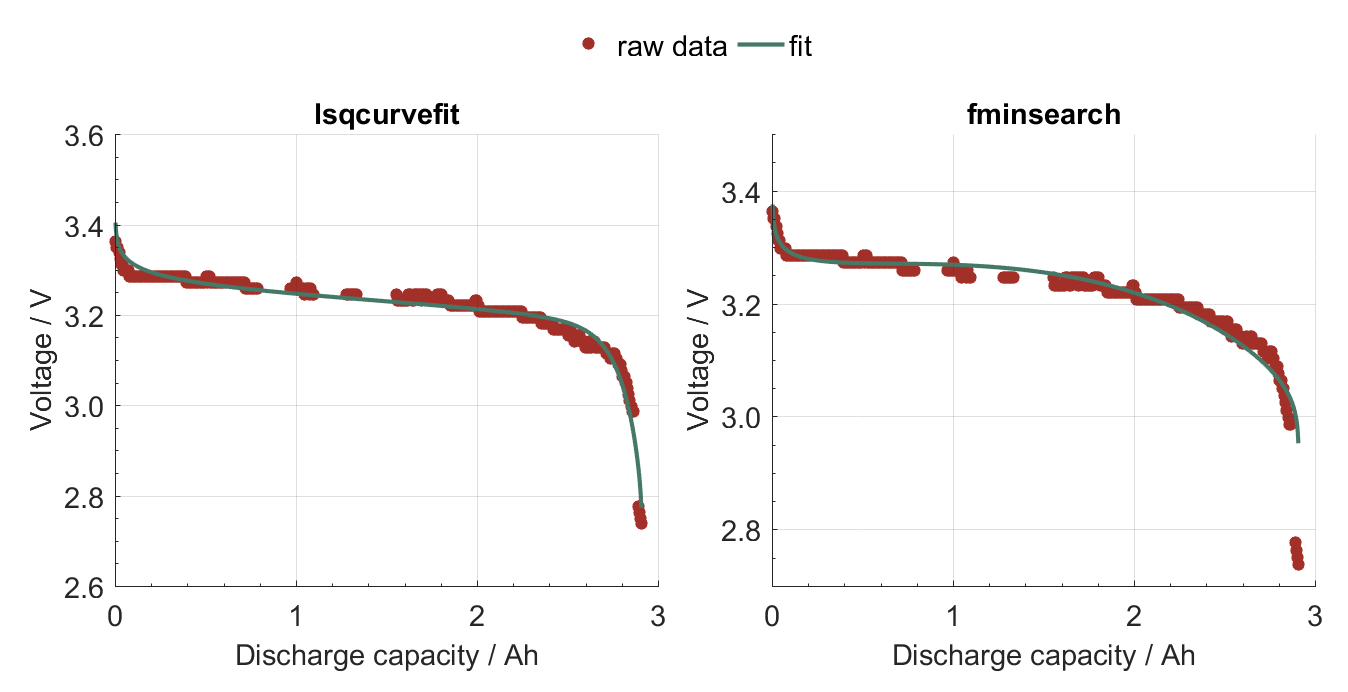
\includegraphics[width=.97\textwidth]{dischargeFit01}
	\caption[Fit results of the \mcode{dischargeFit} class using the fit methods \mcode{lsqcurvefit} and \mcode{fminsearch}, respectively]{Fit results of the \mcode{dischargeFit} class using the fit methods \mcode{lsqcurvefit} and \mcode{fminsearch}, respectively. The raw data was extracted from \cite{_data_2010}.}
	\label{fig:dischargeFit01}
\end{figure}
\begin{figure}[t!]
	\captionsetup{type=figure}
	\centering
	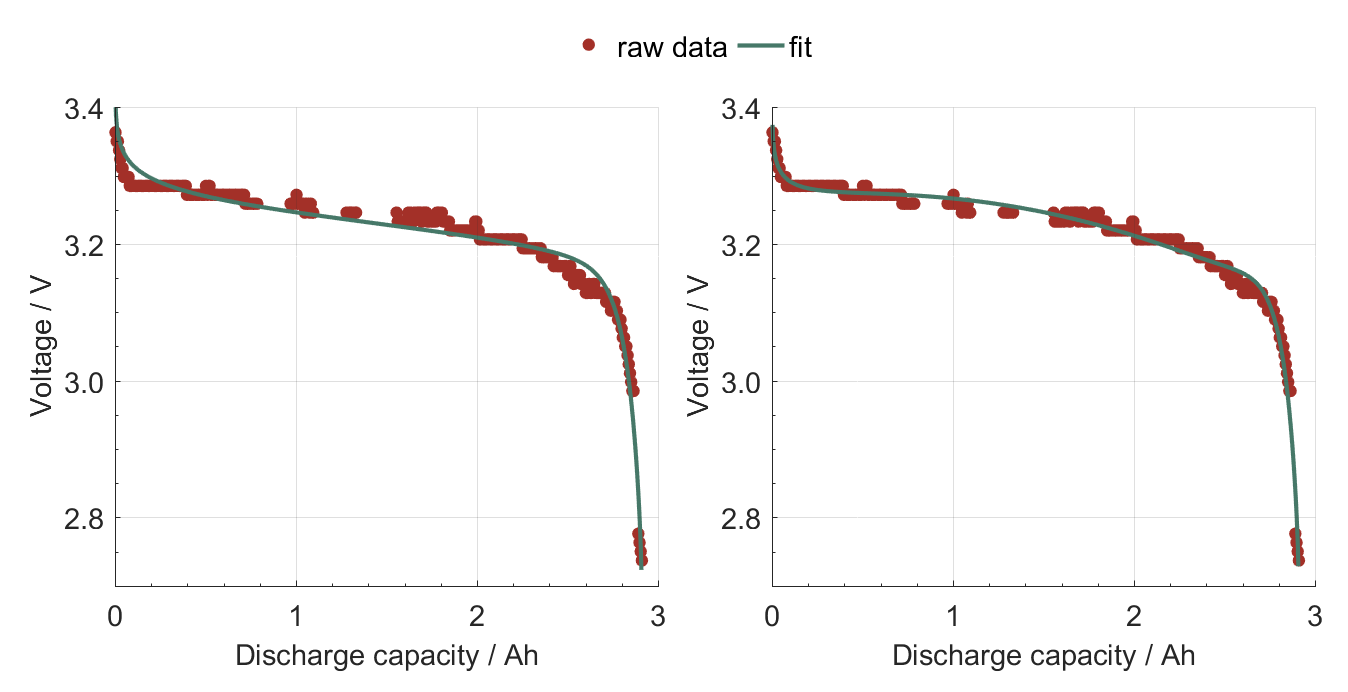
\includegraphics[width=.97\textwidth]{dischargeFit02}
	\caption[Fit results of the \mcode{dischargeFit} class using the fit mode \mcode{'both'} with the default parameter initialization and with a custom parameter initialization]{Fit results of the \mcode{dischargeFit} class using the fit mode \mcode{'both'} with the default parameter initialization (left) and with a custom parameter initialization (right). The raw data was extracted from \cite{_data_2010}.}
	\label{fig:dischargeFit02}
\end{figure}

In this example, \mcode{'lsq'} appears to return better results for the voltage drop at the end of the curve, while \mcode{'fmin'} results in a more precise fit for the voltage drop at the beginning of the curve. Further differences can be seen in the fits' curvatures. 
The \mcode{'lsq'} option results in a slightly flatter curve than the \mcode{'fmin'} mode. The results of a \mcode{dischargeFit} object using the \mcode{'both'} option are presented in Figure~\ref{fig:dischargeFit02}.
Using the default fit parameter initialization of \mcode{zeros} (left) appears to improve the curvature and voltage drops slightly, compared to the other modes. Further improvements can be made by passing custom initial fit parameters to the constructor via the option \mcode{'x0'} (see Figure~\ref{fig:dischargeFit02}, right).

\subsubsection{Object properties}
Further fit quality analysis can be performed via the root mean squared error $rmse$, the mean difference in voltage between the raw data and the curve fit at the respective positions of the raw data $\overline{\Delta V}$ in V and the maximum difference between the raw data and the curve fit at the respective positions $\Delta V\subi{max}$ in V.
The $rmse$ for a curve fit with the raw data $y\subi{raw}$ and the fitted data $y\subi{fit}$ at the same $x$ coordinates is defined as
\begin{equation}
rmse = \sqrt{\sum_{i = 1}^{n}(|y\subs{raw}{i}-y\subs{fit}{i}|)^2}
\end{equation}
where $i$ is the index of the measurement and $n$ is the number of measurements.